% !Mode:: "TeX:UTF-8"


\begin{frame}{第十一讲、全微分与多元复合函数求导}
	\linespread{1.5}
	\begin{enumerate}
	  \item {\bf 内容与要求}{\color{blue}( \S10.2.2-\S10.3.2 )}
	  \begin{itemize}
	    \item 理解全微分的概念
	    \item 熟练掌握多元复合函数的求导方法
	    \item 理解多元函数一阶微分的形式不变性
	  \vspace{1em}
	  \end{itemize}
	  \item {\bf  课后作业:}
	  \begin{itemize}
	    \item {\b 习题10.3:1,2,6,21}
	  \end{itemize}
	\end{enumerate}
\end{frame}

\begin{frame}[<+->]{复习与回顾}
	\linespread{1.5}
	\begin{enumerate}
	  \item {\bf 多元函数的极限与连续}
	  \begin{itemize}
	    \item 多重极限:沿任意路径逼近所得极限相同
	    \item 累次极限存在且相等,多重极限未必存在
	  \end{itemize}
	  \item {\bf 偏导数:}
	  \begin{itemize}
	    \item 对指定变量求导时,将其他变量视为常数
	    \item 偏导存在,未必连续
	    \item 几何意义:沿某坐标轴方向的切线斜率
	  \end{itemize}
	  \item {\bf 高阶偏导:}
	  \begin{itemize}
	    \item 初等函数的高阶偏导与求导次序无关
	  \end{itemize}
	\end{enumerate}
\end{frame}

\section{二元函数的局部线性化}

\begin{frame}{局部线性化}
	\linespread{1.2}\pause 
	\begin{block}{{\bf 一元函数$f(x)$在$x_0$处的微分}\hfill}
		\begin{enumerate}\pause 
		  \item {\bb 可微:}存在常数$A$,使得
		  $$f(x)-f(x_0)=A\Delta x+\circ(\Delta x)$$\pause 
		  \vspace{-2em}
		  \item {\bb 以直代曲:}用$x_0$处的切线近似替代$x_0$附近的函数值\pause 
		  \item {\bb 微分:}
		  $$\d f(x)|_{x=x_0}=A\d x=f'(x_0)\d x$$
		  \vspace{-2em}
		\end{enumerate}
	\end{block}
\end{frame}

\begin{frame}{二元函数的局部线性化}
	\linespread{1.2}\pause 
	\ba{用切平面近似替代$(x_0,y_0)$附近的函数值}\pause 
	
	$$z\approx f(x_0,y_0)+f'_x(x_0,y_0)\Delta x+f'_y(x_0,y_0)\Delta y$$
	
	\pause 
	\alert{{\bf 问题:}}\pause 
	\begin{itemize}
	  \item \alert{在什么情况下,这种近似有意义?}\pause 
	  \item \alert{这种近似蕴含了哪些性质?}
	\end{itemize}
\end{frame}

\begin{frame}
	\linespread{1.2}
	\begin{exampleblock}{{\bf 例1}\hfill}
		求椭圆抛物面$S:z=2x^2+3y^2$在点$P(1,1,5)$处的切平面方程。
	\end{exampleblock}\pause 
	\begin{center}
		\resizebox{!}{4.7cm}{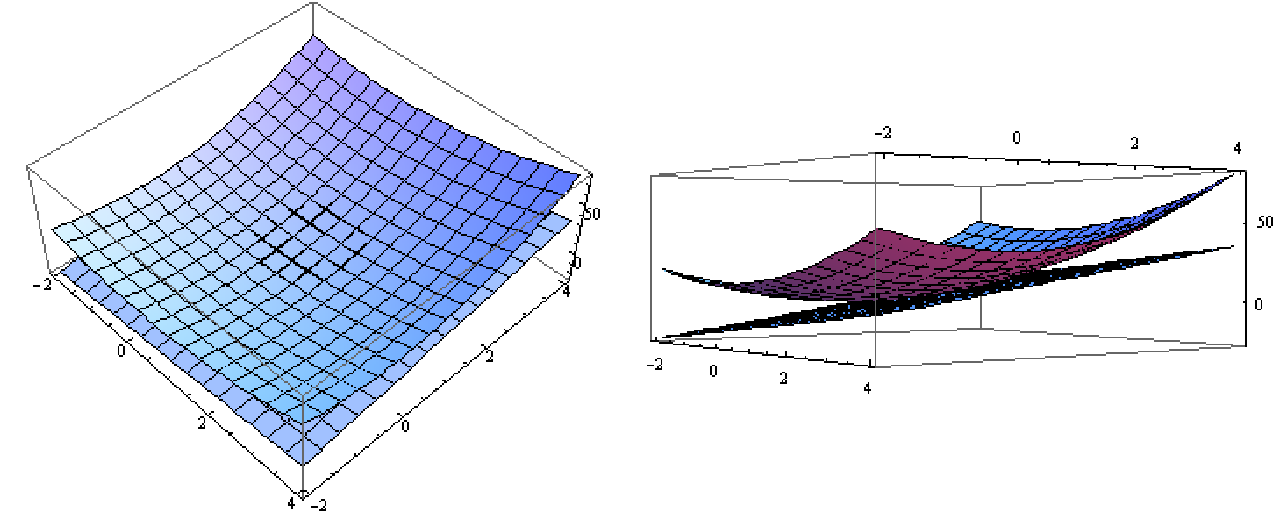
\includegraphics{./images/ch10/tangentFxy.pdf}}
	\end{center}
\end{frame}

\begin{frame}
	\linespread{1.2}
	\begin{exampleblock}{{\bf 例2}\hfill}
		求函数$f(x,y)=\left\{\begin{array}{cc}
			\df{xy}{x^2+y^2},& (x,y)\ne (0,0)\\
			0, & else
		\end{array}\right.$
		在原点处的切平面。
	\end{exampleblock}\pause 
	\begin{center}
		\resizebox{!}{4.5cm}{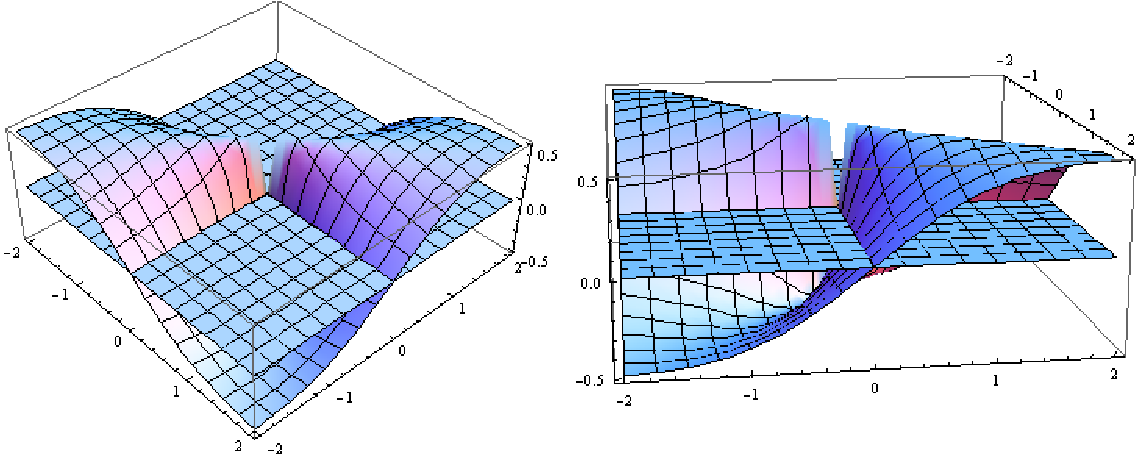
\includegraphics{./images/ch10/tangentNFxy.pdf}}
	\end{center}
\end{frame}

\section{二元函数的全微分}

\begin{frame}{二元函数的全微分}
	\linespread{1.2}\pause 
	\begin{block}{{\bf 定义}\hfill}
		\begin{enumerate}
% 		  \item {\bb 全增量:}
% 			$$\Delta z=f(x_0+\Delta x,y_0+\Delta y)-f(x_0,y_0),$$
% 			其中$\Delta x=x-x_0,\Delta y=y-y_0$
		  \item {\bb 可微:}存在常数$A,B$,使得
		  $$\alert{\Delta z-A\Delta x-B\Delta y=\circ(\sqrt{\Delta x^2+\Delta y^2})}$$
		  \pause \vspace{-2em}
		  \item {\bb 全微分:}
		  $$\alert{\d z|_{(x_0,y_0)}=A\Delta x+B\Delta y}$$
		\end{enumerate}
	\end{block}\pause 
	\begin{exampleblock}{{\bf 例3}\hfill}
		验证$z=2x^2+3y^2$在$(1,1,5)$处可微。
	\end{exampleblock}
\end{frame}

\begin{frame}{二元函数可微的必要条件(1)}
	\linespread{1.2}
	\begin{block}{{\bf 定理10.2.1}\hfill}
		若二元函数$z=f(x,y)$在某点可微,则必在该点连续。
	\end{block}\pause 
	\begin{exampleblock}{{\bf 例4}\hfill}
		函数$f(x,y)=\left\{\begin{array}{cc}
			\df{xy}{x^2+y^2},& (x,y)\ne (0,0)\\
			0, & else
		\end{array}\right.$
		在原点处不可微。
	\end{exampleblock}
\end{frame}

\begin{frame}{二元函数可微的必要条件(2)}
	\linespread{1.2}
	\begin{block}{{\bf 定理10.2.2}\hfill}
		若二元函数$z=f(x,y)$在某点可微,则在该点处的偏导数
		$\df{\p z}{\p x}$和$\df{\p z}{\p y}$均存在,且
		$$\d z=\df{\p z}{\p x}\Delta x+\df{\p z}{\p y}\Delta y$$
	\end{block}\pause 
	\begin{itemize}
	  \item $\alert{\d z=\df{\p z}{\p x}dx+\df{\p z}{\p y}dy}$\pause 
	  \item 偏导数存在,函数不一定可微
	\end{itemize}
\end{frame}

\begin{frame}{二元函数可微的充分条件}
	\linespread{1.2}
	\begin{block}{{\bf 定理10.2.3}\hfill}
		若二元函数$z=f(x,y)$在某点处的偏导函数
		$\df{\p z}{\p x}$和$\df{\p z}{\p y}$连续,则
		$f(x,y)$在该点可微。
	\end{block}
	\pause \bigskip
	\ba{以上所有关于二元函数的结论都可以直接推广到$n$元函数的情形}
\end{frame}

\begin{frame}
	\linespread{1.2}
	\begin{exampleblock}{{\bf 例5}\hfill}
		求$u=e^{x-y}+\sin z$在$(2,1,0)$处的全微分。
	\end{exampleblock}\pause 
	{\bf 小结:}\pause 
	\begin{enumerate}
	  \item 何时可以对曲面进行“以直代曲”?\pause 
	  \begin{itemize}
	    \item \alert{可微$\Leftarrow$偏导函数连续}\pause 
	  \end{itemize}
	  \item 对曲面“以直代曲”意味着什么?\pause 
	  \begin{itemize}
	    \item \alert{曲面“光滑”$\Rightarrow$连续}\pause 
	  \end{itemize}
	  \item 多元函数的微分形式
	  $$\alert{\d z=\df{\p z}{\p x}\d x+\df{\p z}{\p y}\d y}$$
	\end{enumerate}
\end{frame}

\section{多元复合函数求导}

\begin{frame}{多元复合函数求导}
	\linespread{1.2}
	\begin{block}{{\bf 定理10.3.1}(多元函数求导的链式法则)\hfill}
		设$z=f(u,v),u=u(x,y),v=v(x,y)$,\pause 且相关偏导数均存在,\pause 则有
		$$\alert{\df{\p z}{\p x}=\df{\p z}{\p u}\df{\p u}{\p x}
		+\df{\p z}{\p v}\df{\p v}{\p x}}$$\pause \vspace{-1em}
		$$\alert{\df{\p z}{\p y}=\df{\p z}{\p u}\df{\p u}{\p y}
		+\df{\p z}{\p v}\df{\p v}{\p y}}$$
	\end{block}\pause 
	\begin{itemize}
	  \item \ba{“嵌套”$\to$乘积,“并列”$\to$相加}
	\end{itemize}
\end{frame}

\begin{frame}
	\linespread{1.2}
	\begin{exampleblock}{{\bf 例6}\hfill}
		对下列函数分别求$\df{\p z}{\p x}$和$\df{\p z}{\p y}$
		\begin{enumerate}
		  \item $z=e^u\cos v,u=2x-y,v=xy$
		  \item $z=f(3x+2y,x^2+y^2)$
		\end{enumerate}
	\end{exampleblock}
\end{frame}

\begin{frame}{一些典型的情况:}
	\linespread{1.5}\pause 
	\begin{enumerate}
	  \item $z=f(u,v),u=\varphi(x),v=\psi(x)$\pause 
	  \item $z=f(u,v,w),u=u(x,y),v=v(x,y),w=w(x,y)$\pause 
	  \item $z=f(u),u=\varphi(x,y)$\pause 
	  \item $z=f(x,u),u=\varphi(x,y)$
	\end{enumerate}
\end{frame}

\begin{frame}
	\linespread{1.2}
	\begin{exampleblock}{{\bf 例7}\hfill}
		设$z=f(x,x+y,x/y)$,其中$f$可微,求$\df{\p z}{\p x}$和$\df{\p z}{\p y}$
	\end{exampleblock}\pause 
	\begin{exampleblock}{{\bf 例8}\hfill}
		设$z=f(x/y)$,其中$f$可微,证明:$x\df{\p z}{\p x}+y\df{\p z}{\p y}=0$
	\end{exampleblock}\pause 
	\begin{exampleblock}{{\bf 例9}\hfill}
		设$z=xy+xf(x/y)$,其中$f$可微,证明:
		$$x\df{\p z}{\p x}+y\df{\p z}{\p y}=xy+z$$
	\end{exampleblock}
\end{frame}

\begin{frame}
	\linespread{1.2}
	\begin{exampleblock}{{\bf 例10}\hfill}
		设$z=uv+\sin t,u=e^t,v=\cos t$,求$\df{\d z}{\d t}$
	\end{exampleblock}\pause 
	\begin{exampleblock}{{\bf 例11}\hfill}
		设$z=f(xy,x^2-y^2)$,其中$f$具有二阶连续偏导函数,求$\df{\p^2 z}{\p x^2}$和
		$\df{\p^2 z}{\p x\p y}$
	\end{exampleblock}
\end{frame}

\section{一阶微分的形式不变性}

\begin{frame}{一阶微分的形式不变性}
	\linespread{1.2}\pause 
	\ba{一元函数的微分形式不变性:}对于一元函数$f(x)$,无论$x$是自变量
	还是中间变量,其一阶微分形式都是
	$$\d y=f'(x)\d x$$
	\pause 
% 	\vspace{-2em}
	\ba{多元函数的微分形式不变性:}$z=f(\varphi(x,y),\psi(x,y))$的全微分
	$$\alert{\d z=\df{\p z}{\p x}dx+\df{\p z}{\p y}\d y
	=\df{\p z}{\p u}\d u+\df{\p z}{\p v}\d v}$$
	{\bb 无论$u,v$是自变量还是中间变量,其微分形式都一样}
\end{frame}

\begin{frame}{利用微分运算求偏导数}
	\linespread{1.2}
	\begin{exampleblock}{{\bf 例12}\hfill}
		设$z=f(3x+2y,x^2+y^2)$,其中$f$可微,求$\df{\p z}{\p x}$和$\df{\p z}{\p y}$
	\end{exampleblock}
\end{frame}

\begin{frame}[<+->]{小结}
	\linespread{1.5}
	\begin{enumerate}
	  \item {\bf 多元函数的可微与局部线性化}
	  \begin{itemize}
	    \item 可微与连续的关系
	    \item 可微与偏导数的关系
	    \item 微分形式
	  \end{itemize}
	  \item {\bf 复合函数偏导数的计算}
	  \begin{itemize}
	    \item 链式法则:并列+分支
	    \item 利用微分运算求偏导数
	  \end{itemize}
	\end{enumerate}
\end{frame}

% \begin{frame}{title}
% 	\linespread{1.2}
% 	\begin{block}{{\bf title}\hfill}
% 		123
% 	\end{block}
% \end{frame}